\documentclass[conference]{IEEEtran}
\IEEEoverridecommandlockouts
% The preceding line is only needed to identify funding in the first footnote. If that is unneeded, please comment it out.
\usepackage{cite}
\usepackage{amsmath,amssymb,amsfonts}
\usepackage{algorithmic}
\usepackage{graphicx}
\usepackage{textcomp}
\usepackage{xcolor}
\def\BibTeX{{\rm B\kern-.05em{\sc i\kern-.025em b}\kern-.08em
    T\kern-.1667em\lower.7ex\hbox{E}\kern-.125emX}}

%\usepackage{amsmath,amssymb,amsfonts}
%\usepackage{algorithmic}
%\usepackage{graphicx}
%\usepackage{textcomp}
%\usepackage{xcolor}


%\usepackage{cite}
\usepackage{booktabs}   %% For formal tables:
                        %% http://ctan.org/pkg/booktabs
\usepackage{subcaption} %% For complex figures with subfigures/subcaptions
                        %% http://ctan.org/pkg/subcaption
\usepackage{array}
%\usepackage{amsmath,amsfonts}
%\usepackage{algorithm}
%\usepackage[noend]{algpseudocode}
%\usepackage{algorithmic}
%\usepackage{graphicx}
%\usepackage{textcomp}
\usepackage{float}
\usepackage{listings}
\usepackage{xspace}
\usepackage{multirow}
\usepackage{amsthm}
\usepackage{enumitem}

\newtheorem{definition}{Definition}
\usepackage{balance}
\usepackage{printlen}
\usepackage[skins]{tcolorbox}

%\usepackage{xcolor,pifont}
%\newcommand*\colourcheck[1]{%
%	\expandafter\newcommand\csname #1check\endcsname{\textcolor{#1}{\ding{52}}}%
%}
%\colourcheck{blue}
%\colourcheck{green}
%\colourcheck{red}

\newtcolorbox{myframe}[2][]{%
  enhanced,colback=white,colframe=black,coltitle=black,
  sharp corners,
  toprule=1.0pt,
  rightrule=0.3pt,
  leftrule=0pt,
  bottomrule=0pt,
  fonttitle=\itshape\scshape\large,
  left=0pt,right=5pt,top=5pt,bottom=3pt,
  attach boxed title to top right={yshift=-0.3\baselineskip-0.4pt,xshift=-5mm},
  boxed title style={tile,size=minimal,left=0.2mm,right=0.5mm,
    colback=white,before upper=\strut},
  title=#2,#1
}

%\newcommand{\code}[1]{{\footnotesize\textsf{#1}}}

\newcommand{\tool}{\textsc{DeepFQN}\xspace}

\newtheorem{Definition}{Definition}
\newtheorem{Claim}{Claim}
\newtheorem{Lemma}{Lemma}
\newtheorem{Theorem}{Theorem}

\newcolumntype{L}[1]{>{\raggedright\arraybackslash}p{#1}}
\newtheorem{Observation}{Observation}
\newtheorem{property}{Property}
\newcommand{\code}[1]{{\footnotesize\texttt{#1}}}
\usepackage{amsthm}
 \definecolor{dkgreen}{rgb}{0,0.6,0}
\definecolor{gray}{rgb}{0.5,0.5,0.5}
\definecolor{mauve}{rgb}{0.58,0,0.82}
\lstset{frame=tb,
  language=Java,
  aboveskip=3mm,
  belowskip=3mm,
  showstringspaces=false,
  columns=flexible,
  basicstyle={\small\ttfamily},
  numbers=left,
  numberstyle=\tiny\color{gray},
  keywordstyle=\color{blue},
  commentstyle=\color{dkgreen},
  stringstyle=\color{mauve},
  breaklines=true,
  breakatwhitespace=true,
  tabsize=4
}


%\usepackage{tikz}
%\usetikzlibrary{shapes.arrows}
%\newcommand{\FancyUpArrow}{\begin{tikzpicture}[baseline=-0.3em]
%		\node[single arrow,draw,rotate=90,single arrow head extend=0.1em,inner
%		ysep=0.1em,transform shape,line width=0.03em,top color=green,bottom color=green!50!black] (X){};
%\end{tikzpicture}}

%\def\BibTeX{{\rm B\kern-.05em{\sc i\kern-.025em b}\kern-.08em
%    T\kern-.1667em\lower.7ex\hbox{E}\kern-.125emX}}


\begin{document}

%\title{Conference Paper Title*\\
%{\footnotesize \textsuperscript{*}Note: Sub-titles are not captured in Xplore and
%should not be used}
%\thanks{Identify applicable funding agency here. If none, delete this.}
%}

%\makeatletter
%\newcommand{\linebreakand}{%
%\end{@IEEEauthorhalign}
%\hfill\mbox{}\par
%\mbox{}\hfill\begin{@IEEEauthorhalign}
%}
%\makeatother

%\title{Neural Fully-Qualified Name Resolution}
\title{Enabling Fully-Qualified Name Resolution of API Elements via Generative Text Infilling}

%\author{\IEEEauthorblockN{Aashish Yadavally and Tien N. Nguyen}
%\IEEEauthorblockA{\textit{Computer Science Department} \\
%\textit{The University of Texas at Dallas}\\
%Texas, USA \\
%\{aashish.yadavally, tien.n.nguyen\}@utdallas.edu}
%\and
%\IEEEauthorblockN{Wenbo Wang and Shaohua Wang}
%\IEEEauthorblockA{\textit{Department of Informatics} \\
%\textit{New Jersey Institute of Technology}\\
%New Jersey, USA \\
%ww6@njit.edu, davidshwang@ieee.org}
%}

\maketitle

\begin{abstract}
Abstract goes here.
\end{abstract}

%\begin{IEEEkeywords}
%neural partial program analysis, neural program dependence analysis, neural networks; deep learning
%\end{IEEEkeywords}

\section{Introduction}
\label{sec:intro}

Software libraries and frameworks play important roles in software
development. Their functionality is provided via the Application
Programming Interface (API) elements including classes, methods, and
fields. The online forums, e.g., StackOverflow or GitHub Gists, have
provided an excellent resource on how to use API
elements. Unfortunately, due to the current context of the discussions
in such forums, the code snippets in the answering StackOverflow posts
may contain the ambiguities on the references to the API elements of
the external libraries~\cite{liveapi14}.

Several approaches have been proposed to automatically resolve the
fully qualified names (FQNs) of the API elements for the code snippets
in the public forums.  The approaches can be classified into different
categories. The first category is {\em program analysis}. Partial
program analysis~\cite{dagenais-oopsla08} derives the types and FQNs
in a best-effort manner. RecoDoc~\cite{dagenais-icse12} utilizes
several heuristics on syntactic constructs to recognize the names.
The second category is {\em information
  retrieval}. Baker~\cite{liveapi14} builds a candidate list for each
name by tracking the scopes of the names and then overlapping the
lists according to the scoping rules to narrow down the candidates.
COSTER~\cite{coster-ase19} captures the context of the query API
element and matches that with the FQNs of API elements with three
criteria on likelihood, context similarity, and name similarity.  The
third category is {\em constraint-based}.  SnR~\cite{snr-icse22}
builds a knowledge base of APIs, i.e., various facts about the
available APIs.  SnR extracts typing constraints from the given
snippet, and solves the constraints against the knowledge base. The
fourth category leverages the advances in {\em artificial intelligence
  (AI) and machine learning (ML)}. StatType considers the problem of
deriving FQNs as the machine translation from the code without FQNs to
the one with them. Huang {\em et al.}~\cite{prompt-ase22} formulate
the problem as a fill-in-blank task using a masked language model. The
approach fills in the FQN for each name considering the context
consisting of the few lines before and after the fill-in location.
The key issue is that the API elements are designed to use in
different client code, making the surrounding contexts different for
different code using the APIs.

Instead of characterizing the surrounding context
of the fill-in location (i.e., the location of an API element),
we ...


\section{Motivation}
\label{motiv:sec}

\subsection{Motivating Examples}
\label{examples:sec}

%https://stackoverflow.com/questions/4531396/get-value-of-a-edit-text-field/4531500#4531500: SO post #4531500
\begin{figure}[htbp]
	\centering
	\lstset{
		numbers=left,
		numberstyle= \tiny,
		keywordstyle= \color{blue!70},
		commentstyle= \color{red!50!green!50!blue!50},
		frame=shadowbox,
		rulesepcolor= \color{red!20!green!20!blue!20} ,
		xleftmargin=1.5em,xrightmargin=0em, aboveskip=1em,
		framexleftmargin=1.5em,
                numbersep= 5pt,
		language=C,
    basicstyle=\scriptsize\ttfamily,
    numberstyle=\scriptsize\ttfamily,
    emphstyle=\bfseries,
                moredelim=**[is][\color{red}]{@}{@},
		escapeinside= {(*@}{@*)}
	}
\begin{lstlisting}[]
(*@{\color{blue}{Button}@*)   mButton;
EditText mEdit;

(*@@@*)Override public (*@{\color{black}{void}@*) onCreate(Bundle savedInstanceState) {
    super.onCreate(savedInstanceState);
    setContentView(R.layout.main);

    (*@{\color{blue}mButton = findViewById(R.id.button);@*)
    mEdit   = (EditText)findViewById(R.id.edittext);

    (*@{\color{blue}mButton.setOnClickListener(@*)
        (*@{\color{purple}new View.OnClickListener()@*)
        {
            public (*@{\color{black}{void}@*) onClick(View view)
            {
                Log.v("EditText", mEdit.getText().toString());
            }
        });
}
\end{lstlisting}
        \vspace{-12pt}
        \caption{StackOverflow Post \#4531500 on Android Library}
        \label{fig:example1}
\end{figure}


Let us examine some real-world examples to help motivate our approach. Fig.~\ref{fig:example1} illustrates a code snippet of an answer to S/O question \#4531500 on the Android library. Due to the informal discourse in S/O, code snippets rarely contain the necessary declarations and references to the fully-qualified names (FQNs); and often lack the import statements. Besides, the references to external types are also unqualified since the responder assumes that those FQNs can be implicitly understood from the context of the post. For example, in Fig.~\ref{fig:example1}, the types \code{Button} (line 1), \code{EditText} (line 2), \code{Bundle} (line 4), \code{View} (line 14), or \code{Log} (line 16) are referenced only by their simple names. Thus, the code will not be compilable unless the corresponding import statements are added.

%https://stackoverflow.com/questions/18323473/how-to-implement-gwt-java-button-and-the-clickhandler
\begin{figure}[htbp]
	\centering
	\lstset{
		numbers=left,
		numberstyle= \tiny,
		keywordstyle= \color{blue!70},
		commentstyle= \color{red!50!green!50!blue!50},
		frame=shadowbox,
		rulesepcolor= \color{red!20!green!20!blue!20} ,
		xleftmargin=1.5em,xrightmargin=0em, aboveskip=1em,
		framexleftmargin=1.5em,
                numbersep= 5pt,
		language=C,
    basicstyle=\scriptsize\ttfamily,
    numberstyle=\scriptsize\ttfamily,
    emphstyle=\bfseries,
                moredelim=**[is][\color{red}]{@}{@},
		escapeinside= {(*@}{@*)}
	}
\begin{lstlisting}[]
public class myClass implements EntryPoint {
    final (*@{\color{blue}{Button}@*) myButton = new (*@{\color{blue}{Button}@*)("text");
    (*@{\color{blue}{myButton.addClickHandler(}@*)
        (*@{\color{purple}{new ClickHandler() \{}@*)
            public (*@{\color{black}{void}@*) onClick(ClickEvent event) {
               onClickMyButton(event);
        }
    });
    private (*@{\color{black}{void}@*) onClickMyButton(ClickEvent event) {
            ... 
    }
}
\end{lstlisting}
        \vspace{-12pt}
        \caption{StackOverflow Post \#18323473 on GWT Library}
        \label{fig:example2}
\end{figure}


Moreover, the APIs of external libraries are prone to name ambiguity, meaning that they can be confused with other APIs from different libraries that share the same name and offer a similar functionality. For example, the element \code{Button} on line 1 in Fig.~\ref{fig:example1} is a common unqualified type. Here, it refers to \code{android.widget.Button}. Next, consider Fig.~\ref{fig:example2}, which illustrates a code snippet of an answer to a S/O post on Google Web Toolkit (GWT). Because this code snippet does not contain any import statements and the references to the APIs are also unqualified, the type \code{Button} on line 2 in Fig.~\ref{fig:example2} is ambiguous from that on line 1 in Fig.~\ref{fig:example1}. Such name ambiguity in type names is a common phenomenon, especially among S/O code snippets. For instance, the simple name \code{getId} occurs 27,434 times across various Java libraries~\cite{liveapi14}.

\subsection{Observations}
\label{sec:obs}

We can observe a need for a tool that automatically derives the fully-qualified names of the API elements in code snippets from online forums. This will facilitate the reuse of such incomplete code by enabling the addition of the appropriate import statements. To build one such tool, we draw motivation from the following observations.

\vspace{2pt}
\noindent {\bf Observation 1} [{\em Regularity of API Usages}]. The designers of software libraries intend for developers to use the API elements together (including API classes, method calls, and field accesses) in certain combinations/orders to achieve a task. For example, in the GWT code snippet illustrated in Fig.~\ref{fig:example2}, a variable of the type \code{Button} (FQN: \code{com.google.gwt.user.client.ui.Button}) is instantiated on line 2. Then, on line 3, to set the handler of that GWT button, one needs to invoke the \code{addClickHandler} method (FQN: \code{com.google.gwt.user.client.ui.Button.add\-Click\-Handler})  on the \code{Button} object with an argument of the type \code{ClickHandler} (FQN: \code{com\-.google\-.gwt\-.event\-.dom\-.client\-.ClickHandler}). Thus, they are intended to be used in  such a combination and will appear together frequently.

Next, in Fig.~\ref{fig:example3}, we illustrate a complete code example published on the GWT tutorial website \code{gwtproject.org}. Here, the author provides all necessary \code{import} statements and demonstrates how to use different GUI elements in GWT. Specifically, consider the \code{Button} object declared with the \code{addStockButton} variable name on line 12. It calls the method \code{addClickHandler} on line 23 with an argument of the same type as earlier, \code{ClickHandler}. 
%Though the \code{Button} object is assigned with different variable names in both cases, i.e., \code{myButton} when incomplete, and \code{addStockButton} when complete, we can see that the combination of these API elements can help establish its identity in the form of its FQN. 
Despite being assigned with different variable names in both the complete and incomplete cases, i.e., \code{myButton} and \code{addStockButton} respectively, we can see that the combination of these API elements can help establish \code{Button} object's identity and resolve its FQN.

In brief, the source code in public repositories is a good source for a model to implicitly learn the API usages and derive the FQNs of the API elements in an incomplete snippet.

%https://www.gwtproject.org/doc/latest/tutorial/manageevents
\begin{figure}[htbp]
	\centering
	\lstset{
		numbers=left,
		numberstyle= \tiny,
		keywordstyle= \color{blue!70},
		commentstyle= \color{red!50!green!50!blue!50},
		frame=shadowbox,
		rulesepcolor= \color{red!20!green!20!blue!20} ,
		xleftmargin=1.5em,xrightmargin=0em, aboveskip=1em,
		framexleftmargin=1.5em,
                numbersep= 5pt,
		language=C,
    basicstyle=\scriptsize\ttfamily,
    numberstyle=\scriptsize\ttfamily,
    emphstyle=\bfseries,
                moredelim=**[is][\color{red}]{@}{@},
		escapeinside= {(*@}{@*)}
	}
\begin{lstlisting}[]
import com.google.gwt.core.client.EntryPoint;
import com.google.gwt.event.dom.client.ClickEvent;
import com.google.gwt.event.dom.client.ClickHandler;
import com.google.gwt.user.client.ui.Button;
import com.google.gwt.user.client.ui.HorizontalPanel;
import com.google.gwt.user.client.ui.RootPanel;
import com.google.gwt.user.client.ui.VerticalPanel;
...
public class StockWatcher implements EntryPoint {
  private VerticalPanel mainPanel = new VerticalPanel();
  private HorizontalPanel addPanel = new HorizontalPanel();
  private Button addStockButton = new Button("Add");
  ...
  public void onModuleLoad() {
    ...
    // Assemble Add Stock panel.
    addPanel.add(addStockButton);
    // Assemble Main panel.
    mainPanel.add(addPanel);
    // Associate the Main panel with the HTML host page.
    RootPanel.get("stockList").add(mainPanel);
    // Listen for mouse events on the Add button.
    (*@{\color{blue}{addStockButton.addClickHandler(}@*) (*@{\color{purple}{new ClickHandler() \{}@*)
      public void onClick(ClickEvent event) {
        addStock();
      }
    });
  }
  private void addStock() {
    ...
  }
}
\end{lstlisting}
        \vspace{-12pt}
        \caption{Complete Source Code in gwtproject.org}
        \label{fig:example3}
\end{figure}


\vspace{2pt}
\noindent {\bf Observation 2} [{\em Dependencies/Relations among API Elements in a Usage}].
The API elements used together in an API usage in certain combinations/orders share various program dependencies. These relationships can contribute to identifying the FQNs of the API elements better. For example, in Fig.~\ref{fig:example3}, we can see that to set a handler for a button in GWT, the object of the type \code{Button} needs to be the {\em receiving object of the method call} to \code{addClickHandler}, which in turn needs to accept an object of the type \code{ClickHandler} as an argument. The client code utilizing GWT library for this purpose will demonstrate the relationships shared between these three API elements as well. For example, in Fig.~\ref{fig:example2}, if \code{addClickHandler} on line 3 is determined to be the API element \code{com.\-google.\-gwt.\-user.\-client.\-ui.\-Button.\-add\-Click\-Handler}, the FQN of the element at line 4 must be \code{com\-.google\-.gwt\-.event\-.dom\-.client\-.ClickHandler}. The opposite direction of reasoning is also applicable. In general, if a model can learn the dependencies/relations among API elements in an API usage, it could leverage such knowledge to decide the FQNs of all API elements at the same time.

%the lines 2 and 3 in Fig. 2
As another example, consider the data dependency from the \code{def-use} relationship via the variable \code{myButton} between line~2 and line~3 in Fig.~\ref{fig:example2}. This relationship helps derive the FQNs for the above API elements. For instance, if a model decides the FQN for \code{Button} on line 2 to be \code{com\-.google\-.gwt\-.user\-.client\-.ui\-.Button}, it could consequently derive the FQN of \code{add\-Click\-Handler} on line~3 as \code{com.\-google.\-gwt.\-user.\-client.\-ui.\-Button.\-add\-Click\-Handler}, and vice versa.

\vspace{2pt}
\noindent {\bf State-of-the-Art Approaches.} Several approaches have been proposed to recover the fully-qualified names (FQNs) for the API elements in a code snippet. The {\em program-analysis-based} approaches (e.g., PPA~\cite{dagenais-oopsla08}, RecoDoc~\cite{dagenais-icse12}), {\em information-retrieval-based} approaches (e.g., Baker~\cite{liveapi14}, COSTER~\cite{coster-ase19}), and {\em constraint-based} approaches (e.g., SnR~\cite{snr-icse22}) are not comprehensive, and suffer from out-of-vocabulary failures. %(i.e., cannot derive FQNs that were not seen in the training corpus).

Employing the recent advances in {\em machine} and {\em deep learning} (ML \& DL) for FQN resolution has enabled the generation of new FQNs for API elements. However, the state-of-the-art ML/DL-based approaches (e.g., StatType~\cite{icse18} and Huang {\em et al.}~\cite{prompt-ase22}) {\bf do not yet leverage the regularity in API-usages and the dependencies among the relevant API elements} for FQN prediction. StatType~\cite{icse18} leverages phrase-based statistical machine translation to transform an API type-sequence without FQNs to one with them. However, with only short phrases of lengths between 3-8 tokens, StatType is not capable of capturing long-range dependencies between API elements. For example, in Fig.~\ref{fig:example1}, StatType misses the inter-connections between the statements spanning across 11 lines from \code{Button mButton} on line 1 to \code{mButton}, \code{findViewById}, etc. on line 8; and to \code{mButton}, \code{setOnClickListener} on line 11. Moreover, in some cases, it is possible for two relevant API elements to be even farther in the code snippet.

Huang {\em et al.}~\cite{prompt-ase22} formulated FQN resolution as a fill-in-the-blank problem and leveraged a masked language model (MLM\textsubscript{\textit{FIB}}) for this purpose. They build each training instance by taking the statement at each type inference point (e.g., \code{View} on line 12) and a couple of surrounding lines with unresolved API elements as context. This approach has several limitations. First, the amount of contextual information might not capture all relevant API elements corresponding to the same API-usage. In Fig.~\ref{fig:example1}, \code{mButton} on line 1 is far apart from \code{mButton} on line 8 and \code{mButton} on line 11. Next, individual API elements might be used in a different context in the client code. For example, the code on line 9 in Fig.~\ref{fig:example1} is specific to the method \code{onCreate}. Thus, such limited context might not provide the model with sufficient information for determining the FQN.


%Talk about StatType and fill-in


\subsection{Key Ideas}
\label{sec:key}
Following Observations 1--2 and the limitations in existing state-of-the-art approaches, we designed {\tool} to identify the FQNs in a code snippet with the following key ideas:

\vspace{2pt}
\noindent {\bf Key Idea 1} [{\em Leveraging Regularity of API Usages}].
We leverage the pattern-capturing abilities of deep learning models to implicitly learn co-occurring API elements in API usages and derive the FQNs. Observation 1 guides the first principle of our solution, which is the basis of regularity of API usages in the training corpus: the API elements (with their FQNs) appearing together more regularly in API usages have a higher impact on deciding the FQNs than the less regular ones. To facilitate this idea and ensure that the FQNs of all API elements in use are known, we utilize complete, compilable code using libraries from a large code corpus.

\vspace{2pt}
\noindent {\bf Key Idea 2} [{\em ``Tell Me Your Friends, I'll Tell You Who You Are''}].
We consider FQN resolution as a task of identifying inter-connected API elements in a given code snippet. As described in Observation 2, rather than attempting to determine the FQN of an API element based solely on its individual characteristics (e.g., local surrounding context) as in the state-of-the-art approach Huang {\em et al.}~\cite{prompt-ase22}, we adopt a broader dependency context that include program dependencies and inter-API relationships. Based on this knowledge, we aim to derive all related API elements simultaneously.

%We use a graph representation, called Augmented Usage Graph
%(AUG)~\cite{msr19}, to represent the program dependencies and
%relations among program entities and API elements. We extract the AUGs
%from the complete, compilable source code using the APIs from a large
%code corpus. We then enhance the AUGs with all the FQNs because the
%training code is compilable. From those AUGs,

\vspace{2pt}
\noindent {\bf Key Idea 3} [{\em FQN Resolution via Text Infilling}].
Deriving FQNs in an incomplete code snippet can be postulated as a fill-in-the-blank task, wherein the missing parts of a fully-qualified name are inserted ahead of its corresponding simple name at all relevant type inference locations. For example, in Fig.~\ref{fig:example3}, a blank representing \code{com.google.gwt.event.dom.client} will be inserted ahead of \code{ClickEvent}. To fill in all such inserted blanks, we adopt a Causal Language Model (CLM) capable of generating text and extend its capabilities to predict the missing spans of text in the blanks. Let us call this framework an Infilling Language Model (ILM). The blanks thus constructed are consistent with the preceding and subsequent code, thus enabling the ILM to gain access to the wider dependency context and learn from the interconnections among the API and program elements in the code snippet.


%\section{Important Concepts}
\label{sec:concepts}

This section describes the definitions of the important concepts
regarding our representations on API usages.

\begin{figure}[t] %[!htp]
	\centering
	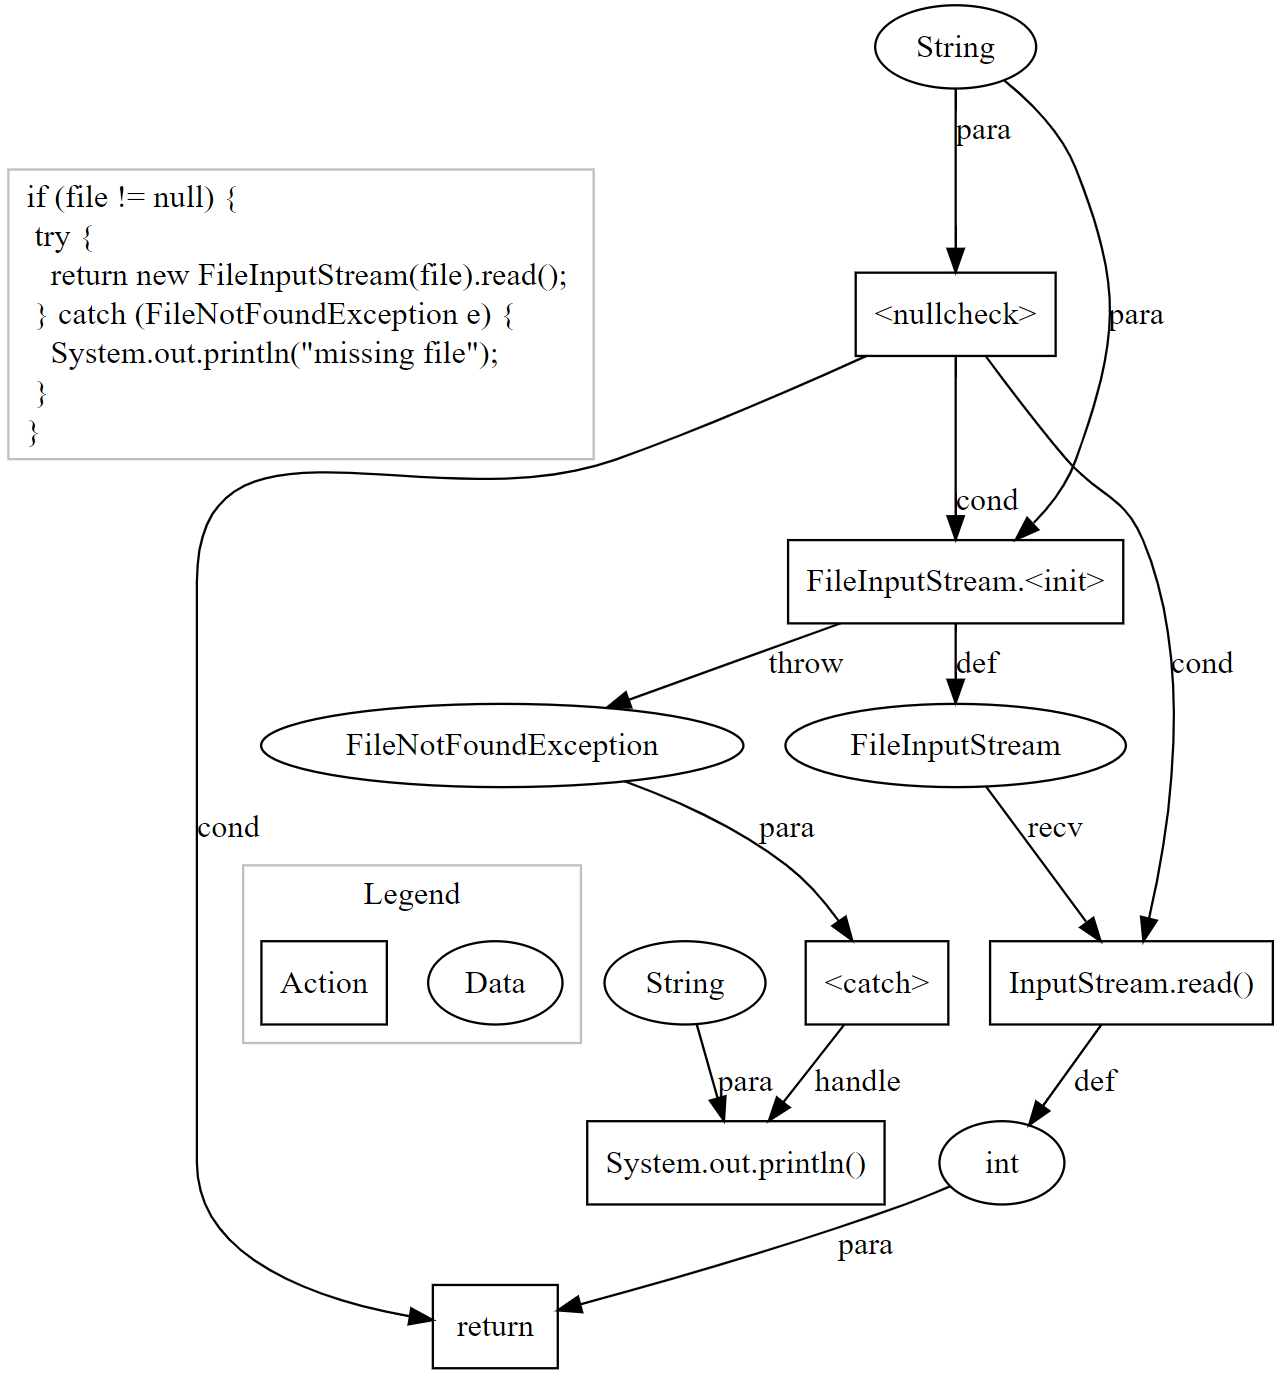
\includegraphics[width=0.9\linewidth]{aug-example}
        \vspace{-3pt}
	\caption{An API Usage and its API-Usage Graph}
	\label{fig:aug}
\end{figure}

\begin{Definition}[API elements]
  An API element is either a class, a method, or a field that is
  provided in a library to enable the accesses to the library's
  functions via a variable declaration with a certain class, a method
  call to an API method, or a field access to an API field.
\end{Definition}

For example, in Figure~\ref{fig:example3}, line 12, \code{Button} is
an API class, which is a declared type for the variable
\code{addStockButton}. At line 23, \code{addClickHandler} is an API
method, which is called on the variable \code{addStockButton}.

\begin{Definition}[API Usage]
An API usage consists of a set of API elements and control structures
(i.e., conditions and repetitions), together with other program
elements (e.g., variables, parameters, etc.) in specific combinations
and orders to perform a programming task.
\end{Definition}

In Figure~\ref{fig:example2}, lines 2-4 show an API usage consisting
of 1) a variable \code{myButton}, 2) its declared class \code{Button},
3) a method call to \code{addClickHandler} on the variable
\code{myButton}, 4) the method call \code{add\-Click\-Handler} accepting an
argument of the type \code{ClickHandler}, etc.

\begin{Definition}[API Usage Relation]
  In an API usage, there exist the API usage relations among the API
  elements and relevant program elements. The API usage relations
  include the following ones: {\bf receiver, parameter, definition,
    order, condition, synchronize, throw, handle}, and {\bf data and
    control dependencies} among the API and program elements (will be
  detailed next).
\end{Definition}

Let us use the term {\em action nodes} to refer to method calls, field
accesses, or operators, and the term {\em data nodes} to represent
objects, values, and literals that appear in API usages. A {\em
  receiver} relation exists between a variable and a method call. In
Figure~\ref{fig:example2}, at line 3, there exists a receiver relation
between the variable \code{myButton} and the method
\code{addClickHandler}. A {\em parameter} relation connects an
argument to be used as a parameter of an action. A {\em definition}
relation exists between a constructor or method call that creates or
returns a value or object to the respective variable. An {\em order}
relation connects two actions on operating on the same receiver or
parameter. A {\em condition} relation connects an action whose result
controls branching to an action being controlled. A {\em synchronize}
relation connects a variable that the program obtains a lock on to an
action executed under that lock. A {\em throw} relation connects an
action that may throw an exception to a data node representing that
exception object. A {\em handle} relation connects from a \code{catch}
action to an action in a respective exception handling block.

We expect to leverage those API usage relations among the API elements
and relevant program entities to identify the FQNs. Toward that goal,
we adopt a graph-based representation for API usages, called {\em
  API-Usage Graphs (AUGs)}~\cite{msr19}.

\begin{Definition}[API Usage Graph (AUG)~\cite{msr19}]
AUG is a directed, connected graph with labelled nodes and
edges. Nodes represent data entities (variables, values), and actions,
(e.g., method calls or operators). Edges represent the API usage
relations
%as well as control and data dependencies
among the entities and actions represented by nodes.
\end{Definition}

Figure~\ref{fig:aug} shows an example of an API usage and its AUG.
The action nodes are displayed in the rectangles and the data nodes in
the oval shapes. The action nodes represent constructor calls
(\code{init}), method calls, field accesses, and operators. If the
types are available, they will be resolved. However, in the figure,
only the simple name is shown for clarity. The relational operators
are also encoded as actions to capture conditions. The data nodes
represent objects, values, and literals in an API usage. AUG encodes
data entities as nodes to make explicit the data dependencies between
actions, such as multiple calls on the same object to ensure we have a
connected subgraph with all data-dependent parts of a usage. The usage
relations are shown with their labels. {\em Order} edges are not
shown for clarity. The AUG building algorithm is explained in~\cite{msr19}.


\section{Approach Overview}
\label{sec:overview}



\section{Our Approach}
\label{sec:approach}

\subsection{Type Inference Location Extraction}
\subsubsection{AST Parsing} As a first step towards building \code{<blank>}-sequences, we need to build the AST for a given code snippet. In cases where it is complete, constructing an AST is trivial. In cases where it is incomplete, we can utilize tools such as PPA~\cite{} to build an AST in a best-effort manner.

\subsubsection{Node Transformation}

\subsubsection{AST Unparsing}



Next, we traverse the AST and transform the source code corresponding to each of the type-specific AST nodes as follows:

%\begin{enumerate}[label=\roman*.]
    \item \textbf{Array Creation}

    \textit{Formal Syntax:} \code{new TypeName [ < Type { , Type } > ] [ Expression ] {[ Expression ]} { [ ] }}

    \textit{Syntax:} \code{new TypeName [ < Type { , Type } > ] [ Expression ] {[ Expression ]} { [ ] }}
    
    \textit{Transformation:}    
    %%%%%%%%%%%%%%%%%%%%%%%%%%%%%%%%%%%%%%%%%%%%%%%%%%%%%%%%%    
    \item \textbf{Cast Expression}

%    \textit{Formal Syntax:} \code{( Type ) Expression}
 
    $(\mathcal{N}_{\mathcal{S}}) E \rightsquigarrow (\text{\code{<blank>}. }\mathcal{N}_{\mathcal{S}}) E$    
    %%%%%%%%%%%%%%%%%%%%%%%%%%%%%%%%%%%%%%%%%%%%%%%%%%%%%%%%%  
    \item \textbf{Class Instance Creation}

%    \textit{Formal Syntax:} \code{new [ < Type { , Type } > ] Type ( [ Expression { ,  Expression } ] )}

    $\text{\textbf{\code{new}} }\mathcal{N}_{\mathcal{S}}(E_1, E_2, ..., E_n) \rightsquigarrow\text{ \textbf{\code{new}} \code{<blank>}. }\mathcal{N}_{\mathcal{S}}(E_1, E_2, ..., E_n)$    
    %%%%%%%%%%%%%%%%%%%%%%%%%%%%%%%%%%%%%%%%%%%%%%%%%%%%%%%%%    
    \item \textbf{Instanceof Expression}

%    \textit{Formal Syntax:} \code{Expression instanceof Type}
    
    $E\text{ \textbf{\code{instanceof}} }(\mathcal{N}_{\mathcal{S}}) \rightsquigarrow E\text{ \textbf{\code{instanceof}} }( \text{\code{<blank>}. }\mathcal{N}_{\mathcal{S}})$
    %%%%%%%%%%%%%%%%%%%%%%%%%%%%%%%%%%%%%%%%%%%%%%%%%%%%%%%%%    
%    \item \textbf{Single Variable Declaration}
%
%    \textit{Syntax:} \code{{ ExtendedModifier } Type {Annotation} [ ... ] Identifier { Dimension } [ = Expression ]}
%    
%    \textit{Transformation:}
    %%%%%%%%%%%%%%%%%%%%%%%%%%%%%%%%%%%%%%%%%%%%%%%%%%%%%%%%%    
    \item \textbf{(Super) Constructor Invocation}

%    \textit{Formal Syntax:} \code{< this | super > ( [ Expression { , Expression } ] ) ;}

    $\{\text{\textbf{this}}\vert\text{\textbf{super}\}}(E_1, E_2, ..., E_n) \rightsquigarrow \text{\code{<blank>} }(E_1, E_2, ..., E_n)$    
    %%%%%%%%%%%%%%%%%%%%%%%%%%%%%%%%%%%%%%%%%%%%%%%%%%%%%%%%%    
    \item \textbf{(Super) Field Access}

%    \textit{Syntax:} \code{Expression . Identifier}

%    \textit{Syntax:} \code{super . Identifier}

    $\{E\vert\text{\textbf{super}\}}.I \rightsquigarrow \text{\code{<blank>}. }I$
    %%%%%%%%%%%%%%%%%%%%%%%%%%%%%%%%%%%%%%%%%%%%%%%%%%%%%%%%%    
    \item \textbf{(Super) Method Invocation}

%    \textit{Syntax:} \code{Identifier ( [ Expression { , Expression } ] )}

%    \textit{Syntax:} \code{super . Identifier ( [ Expression { , Expression } ] )}
    
    $\{I\vert\text{\textbf{super}.}I\}(E_1, E_2, ..., E_n) \rightsquigarrow \text{\code{<blank>}. }I(E_1, E_2, ..., E_n)$
    %%%%%%%%%%%%%%%%%%%%%%%%%%%%%%%%%%%%%%%%%%%%%%%%%%%%%%%%%    
    \item \textbf{Throw Statement}

%    \textit{Syntax:} \code{throw Expression ;}
    
    $\text{\textbf{\code{throw }}}\mathcal{N}_{\mathcal{S}} \rightsquigarrow \text{\textbf{\code{throw }}\code{<blank>}. }\mathcal{N}_{\mathcal{S}}$
    %%%%%%%%%%%%%%%%%%%%%%%%%%%%%%%%%%%%%%%%%%%%%%%%%%%%%%%%%    
\end{enumerate}
% Please add the following required packages to your document preamble:
% \usepackage{multirow}
\begin{table*}[]
\centering
\begin{tabular}{l|c}
\toprule
\multicolumn{1}{c|}{\textbf{Node Type}}                               & \textbf{Transformation Rule and Example}                                                                                                                                                              \\ \hline
\multirow{3}{*}{Array Creation}                 & \cellcolor{gray!15} $\text{\tabcode{\textbf{new }}}\mathcal{N}_\mathcal{S}[E] \:\rightsquigarrow\: \text{\tabcode{\textbf{new }<blank>.}}\mathcal{N}_\mathcal{S}[E]$  \\
                                                & \multicolumn{1}{l}{\textit{Example}: \tabcode{new Context[contexts.size()]} $\:\rightsquigarrow\:$ \tabcode{new <blank>.Context[contexts.size()]}} \\ 
                                                & \multicolumn{1}{l}{\textit{FQN}: \tabcode{org.xml.sax.helpers.NamespaceSupport}} \\ \hline
\multirow{3}{*}{Cast Expression}                & \cellcolor{gray!15} $(\mathcal{N}_{\mathcal{S}}) E \:\rightsquigarrow\: (\text{\tabcode{<blank>}. }\mathcal{N}_{\mathcal{S}}) E$                                                                                \\
                                                & \multicolumn{1}{l}{\textit{Example}: \tabcode{(LexicalHandler) value} $\:\rightsquigarrow\:$ \tabcode{(<blank>.LexicalHandler) value}} \\ 
                                                & \multicolumn{1}{l}{\textit{FQN}: \tabcode{org.xml.sax.ext}} \\ \hline
\multirow{2}{*}{Class Instance Creation}        & \cellcolor{gray!15} $\text{\textbf{\tabcode{new}} }\mathcal{N}_{\mathcal{S}}(E_1, E_2, ..., E_n) \:\rightsquigarrow\:\text{ \textbf{\tabcode{new}} \tabcode{<blank>}. }\mathcal{N}_{\mathcal{S}}(E_1, E_2, ..., E_n)$ \\
                                                & \multicolumn{1}{l}{\textit{Example}: \tabcode{new Context()} $\:\rightsquigarrow\:$ \tabcode{new <blank>.Context()}} \\ 
                                                & \multicolumn{1}{l}{\textit{FQN}: \tabcode{org.xml.sax.helpers.NamespaceSupport}} \\ \hline
\multirow{3}{*}{Instanceof Expression}          & \cellcolor{gray!15} $E\text{ \textbf{\tabcode{instanceof}} }\mathcal{N}_{\mathcal{S}} \:\rightsquigarrow\: E\text{ \textbf{\tabcode{instanceof}} } \text{\tabcode{<blank>}. }\mathcal{N}_{\mathcal{S}}$           \\
                                                & \multicolumn{1}{l}{\textit{Example:} \tabcode{addr instanceof Inet6Address} $\:\rightsquigarrow\:$ \tabcode{addr instanceof <blank>.Inet6Address}} \\ 
                                                & \multicolumn{1}{l}{\textit{FQN}: \tabcode{java.net}}\\\hline
\multirow{3}{*}{Single Variable Declaration}    & \cellcolor{gray!15}  $\mathcal{N}_\mathcal{S}\text{ }I\:\{\:= E\} \:\rightsquigarrow\:$ $\text{\tabcode{<blank>}. }\mathcal{N}_\mathcal{S}\text{ }I\:\{\:= E\}$\\
                                                & \multicolumn{1}{l}{\textit{Example}: \tabcode{Node<E> x} $\:\rightsquigarrow\:$ \tabcode{<blank>.Node<E> x}} \\ 
                                                & \multicolumn{1}{l}{\textit{FQN}: \tabcode{java.util.concurrent.LinkedBlockingDeque}} \\ \hline
\multirow{3}{*}{(Super) Constructor Invocation} & \cellcolor{gray!15} $\{\text{\textbf{\tabcode{this}} }\vert\text{ \textbf{\tabcode{super}}\}}(E_1, E_2, ..., E_n) \:\rightsquigarrow\: \text{\tabcode{<blank>} }(E_1, E_2, ..., E_n)$                                                 \\
                                                & \multicolumn{1}{l}{\textit{Example}: \tabcode{this(address, true)} $\:\rightsquigarrow\:$ \tabcode{<blank>(address, true)}} \\ 
                                                & \multicolumn{1}{l}{\textit{FQN}: \tabcode{org.apache.harmony.tests.java.net.DatagramSocketTest.DatagramServer}}\\ \hline
\multirow{3}{*}{(Super) Field Access}           & \cellcolor{gray!15} $\{E\text{ }\vert\text{ \textbf{\tabcode{super}}\}}.I \:\rightsquigarrow\: \text{\tabcode{<blank>}. }I$                                                                                                        \\
                                                & \multicolumn{1}{l}{\textit{Example}: \tabcode{this.changeConfig} $\:\rightsquigarrow\:$ \tabcode{<blank>.changeConfig}}               \\ 
                                                & \multicolumn{1}{l}{\textit{FQN}: \tabcode{android.compat.Compatibility.OverrideCallbacks}} \\ \hline
\multirow{3}{*}{(Super) Method Invocation}      & \cellcolor{gray!15} $\{I\text{ }\vert\text{\textbf{ \tabcode{super}}.}I\}(E_1, E_2, ..., E_n) \:\rightsquigarrow\: \text{\tabcode{<blank>}. }I(E_1, E_2, ..., E_n)$                                                                \\
                                                & \multicolumn{1}{l}{\textit{Example}: \tabcode{connectLocalServer()} $\:\rightsquigarrow\:$ \tabcode{<blank>.connectLocalServer()}}      \\ 
                                                & \multicolumn{1}{l}{\textit{FQN}: \tabcode{org.apache.harmony.tests.java.nio.channels.DatagramChannelTest}}\\
% \multirow{2}{*}{Throw Statement}                & \cellcolor{gray!15} $\text{\textbf{\tabcode{throw }}}E \:\rightsquigarrow\: \text{\textbf{\tabcode{throw }}\tabcode{<blank>}. }\mathcal{N}_{\mathcal{S}}$                                     \\
%                                                 & \multicolumn{1}{l}{\textit{Example}: \tabcode{} $\:\rightsquigarrow\:$ \tabcode{}} \\ 
%                                                 & \multicolumn{1}{l}{\textit{FQN}: \tabcode{}} \\
\bottomrule
\end{tabular}
\caption{AST node-level transformation rules for constructing \tabcode{<build>}-sequences in Type Inference Location Extraction (TILE) algorithm. Here, $\mathcal{N}_\mathcal{S}$ denotes \textit{Simple Name}, $E_i$ denotes \textit{Expression}, and $I$ denotes \textit{Identifier}.}
\end{table*}

\subsection{Type Inference with Infilling Language Model}
\subsubsection{Problem Formulation}

\subsubsection{Training Process}

\subsubsection{Inference}



\section{Empirical Evaluation}
\label{sec:evaluation}

%\subsection{Research Questions}

We conducted several experiments to evaluate {\tool}. We aim to answer the following questions:

\vspace{2pt}
\noindent \textbf{RQ\textsubscript{1} 
  [Effectiveness Evaluation]} {\em How accurate is {\tool} in expanding FQNs for complete code from Java projects?}

\vspace{2pt}
\noindent \textbf{RQ\textsubscript{2}
[API-Usage Relations]} {\em Do the conditioning-driven interactions help the model learn API usages?}

\vspace{2pt}
\noindent \textbf{RQ\textsubscript{3} 
[Ablation Study]}  {\em Is there a benefit to leveraging a wider dependency context in comparison to a narrower surrounding context for predicting fully qualified names?}

%{\em Is our tool capable of capturing the API-usage relations between API elements and other program elements in the code snippet?}

% \vspace{2pt}
% \noindent \textbf{RQ\textsubscript{4} 
% [Practicality Evaluation]}  {\em How accurate is {\tool} in 
% inferring FQNs for API elements in incomplete code snippets from online forums such as StackOverflow?}

%\subsection{Empirical Methodology}

\subsubsection{Datasets}

\subsubsection{RQ1.}

{\em Baselines.}

{\em Procedure.}

{\em Tuning.}

{\em Metrics.}

\subsubsection{RQ2.}

{\em Baselines.}

{\em Procedure.}

{\em Tuning.}

{\em Metrics.}



\section{Effectiveness Evaluation}
\label{sec:effectiveness-eval}

\subsection{Data Collection}\label{sec:effectiveness-data}

% Please add the following required packages to your document preamble:
% \usepackage{multirow}
\begin{table}[t]
\centering
%\scriptsize
\begin{tabular}{c|cc|cc|cc}
\toprule
%\multirow{2}{*}{\diagbox{\textbf{Project} ($\downarrow$)}{\textbf{Split} ($\rightarrow$)}}                 & \multicolumn{2}{c|}{\textbf{Train}}         & \multicolumn{2}{c|}{\textbf{Validation}}    & \multicolumn{2}{c}{\textbf{Test}}           \\ \cline{2-7}
% \multirow{2}{*}{\diagbox{\textbf{Project}}{\textbf{Split}}}                 & \multicolumn{2}{c|}{\textbf{Train}}         & \multicolumn{2}{c|}{\textbf{Validation}}    & \multicolumn{2}{c}{\textbf{Test}}           \\ \cline{2-7}
\multicolumn{1}{r|}{\textbf{Split} ($\rightarrow$)}    & \multicolumn{2}{c|}{\textbf{Train}}         & \multicolumn{2}{c|}{\textbf{Validation}}    & \multicolumn{2}{c}{\textbf{Test}}           \\ \cline{2-7}
\multicolumn{1}{l|}{\textbf{Library} ($\downarrow$)}   & \multicolumn{1}{c|}{$N_x$} & $N$\textsubscript{API} & \multicolumn{1}{c|}{$N_x$} & $N$\textsubscript{API} & \multicolumn{1}{c|}{$N_x$} & $N$\textsubscript{API} \\
\hline
\code{android}   & \multicolumn{1}{c|}{2,389}             &  10,878       & \multicolumn{1}{c|}{298}             & 1,273        & \multicolumn{1}{c|}{300}             &  1,285       \\
\tabcode{gwt}       & \multicolumn{1}{c|}{33,954}             & 191,946        & \multicolumn{1}{c|}{4,244}             &  23,991       & \multicolumn{1}{c|}{4,245}             & 23,937        \\
\code{hibernate} & \multicolumn{1}{c|}{52,910}             & 171,496        & \multicolumn{1}{c|}{6,613}             & 22,173        & \multicolumn{1}{c|}{6,615}             & 22,074        \\
\code{jdk}       & \multicolumn{1}{c|}{3,124}             & 11,994        & \multicolumn{1}{c|}{390}             &  1,339       & \multicolumn{1}{c|}{392}             & 1,398        \\
\code{joda-time} & \multicolumn{1}{c|}{4,976}             &  13,396       & \multicolumn{1}{c|}{622}             &  1,754       & \multicolumn{1}{c|}{623}             & 1,606        \\
\code{xstream}   & \multicolumn{1}{c|}{2,774}             &  7,909       & \multicolumn{1}{c|}{346}             &  1,120       & \multicolumn{1}{c|}{348}             &  995       \\ \hline
\textbf{Total}   & \multicolumn{1}{c|}{100,127}             & 407,619        & \multicolumn{1}{c|}{12,513}             & 51,650        & \multicolumn{1}{c|}{12,523}             & 51,395        \\ 
\bottomrule
\end{tabular}
\caption{Dataset statistics. $N_x$: the number of data instances; $N$\textsubscript{API}: the number of API elements.}
\label{tab:data-stats}
\end{table}

%% Total instances: android - 2987, gwt - 42443, hibernate-orm 66138, jdk 3906, joda-time 6221, xstream 3468
%% Total APIs: android - 13536, gwt - 239874, hibernate-orm 215743, jdk 14931, joda-time 16756, xstream 10024
%% Unique APIs: android - 569, gwt - 5949, hibernate - 12618, jdk - 1480, joda-time - 401, xstream - 643


To enable the effectiveness evaluation, we considered six popular Java libraries that developers typically make use of: \code{android}, \code{gwt}, \code{hibernate}, \code{jdk}, \code{joda-time}, and \code{xstream}. This is consistent with prior works on FQN resolution~\cite{icse18, snr-icse22, prompt-ase22}. Among these, StatType\cite{icse18} and SnR\cite{snr-icse22} leverage projects that utilize these libraries. A limitation with this approach is that not all library API elements are covered in their dataset. In contrast, we download these large-scale repositories from GitHub and use their source code itself to build our dataset.

We used Eclipse JDT to parse each project’s source code and resolve all the FQNs. Next, we traversed the ASTs to collect all the methods. Overall, these libraries contain 198,231 methods including 9,764 from \code{android}, 62,782 from \code{gwt}, 105,734 from \code{hibernate-orm}, 5,235 from \code{jdk}, 9,811 from \code{joda-time}, and 4,905 from \code{xstream}. Next, we randomly split these in a 80\%-10\%-10\% ratio, each for training, validation, and testing, respectively. Finally, we applied the TILE algorithm to identify the type inference locations and build the $\langle$\blank-code, FQN$\rangle$ pairs, discarding the methods with no such pairs. In general, we have 125,163 instances carrying 510,664 FQNs. Among these, 58,543 API elements carry unique FQNs, and 21,660 carry unique FQN prefixes (i.e., unresolved part of the FQN). We report the fine-grained library/split-level data statistics in Table~\ref{tab:data-stats}.

\subsection{Procedure \& Evaluation Metrics}\label{sec:effectiveness-eval-proc}
We design this experiment to test the effectiveness of \tool in resolving FQNs in complete code. For all experiments, we train the same CLM, i.e., GPT-2 “small” (containing 124M parameters) within the ILM framework.

\noindent\underline{\textit{Baselines}}: Due to the formulation of our approach as a fill-in-the-blank task, we can establish a direct comparison with the following: (a) off-the-shelf CodeBERT model (MLM\textsubscript{\textit{base}})~\cite{codebert}, (b) prompt-tuned CodeBERT model (MLM\textsubscript{\textit{FIB}})~\cite{prompt-ase22}. Besides, Huang et al. reported that reserving 30\% of the data for the prompt-tuning phase gives them stable model performance. Accordingly, for MLM\textsubscript{\textit{FIB}}, we reserve 30\% of our training data for prompt-tuning, and remaining 70\% for fine-tuning.

\noindent\underline{\textit{Data Preparation for Baselines}}: We followed the FQN prompt generation steps detailed in \cite{prompt-ase22} to build the training data for both prompt-tuning and fine-tuning phases in MLM\textsubscript{\textit{FIB}}. Due to the code fragmentation step in MLM\textsubscript{\textit{FIB}}, each training instance with $k$ type inference points in our dataset (i.e., at the method-level) corresponds to $k$ prompts/training instances for this baseline. Note that whole FQNs in a prompt are masked during the prompt-tuning phase, while the FQN prefixes are masked in the fine-tuning phase.

\noindent\underline{\textit{FQN Resolution with Baselines}}: In MLM\textsubscript{\textit{base}}, there is no additional training required since we use CodeBERT off-the-shelf. In MLM\textsubscript{\textit{FIB}}, CodeBERT is first prompt-tuned, then fine-tuned for enabling FQN resolution. An MLM is not designed to handle variable lengths of missing spans, and needs to know the length of the FQN prefix (i.e., the number of sub-tokens it corresponds to) beforehand. However, this is presumably not available during the inference phase. Huang et al. address this issue by producing multiple prompts with the lengths of FQNs ranging from the minimum mask span (i.e., 2) and the maximum mask span (i.e., 52), and select the FQN prefix prediction with the highest average probability. We followed suit to establish the inference process with both the baselines.

\noindent\underline{\textit{Evaluation Metrics}}: We use the following metrics to assess the model performance: (a) \textit{Exact Match Accuracy} (Accuracy\textsubscript{EM}), a stricter version of accuracy which ensures that the predicted FQN is exactly the same as the ground-truth FQN; (b) \textit{ROUGE-L}\footnote{Given ground-truth FQN $X$ and predicted FQN $Y$ of lengths $x$ and $y$, respectively: Recall, $R_{LCS}=\frac{LCS(X, Y)}{x}$, Precision, $P_{LCS}=\frac{LCS(X, Y)}{y}$, and F-measure, $F_{LCS}=\frac{2.R_{LCS}.P_{LCS}}{R_{LCS}+P_{LCS}}$.}, which compares the similarity between the predicted FQN and the ground-truth FQN based on the longest common subsequence (LCS); and (c) \textit{BLEU-2}, which compares the similarity between the predicted FQN and the ground-truth FQN based on bigrams in the subword tokens.

\subsection{RQ1... }
\label{sec:rq1}



\section{Investigating API-Usage Relation Learning }
\label{sec:eval}

% \subsection{Background, and Data Collection}
% \subsection{Experiment Methodology}
% \subsection{Evaluation Metrics}
%\subsection{Experiment Results (RQ\textsubscript{3})}
\label{sec:rq3}

% Please add the following required packages to your document preamble:
% \usepackage{multirow}
\begin{table}[]
\centering
\begin{tabular}{l|ccc}
\toprule
\multirow{2}{*}{\textbf{Approach}} & \multicolumn{3}{c}{\textbf{Metrics}}                                  \\ \cline{2-4} 
                                   & \multicolumn{1}{c|}{\textit{Accuracy\textsubscript{EM}}} & \multicolumn{1}{c|}{\textit{ROUGE-L}} & \textit{BLEU-2} \\ \hline
\multicolumn{1}{c|}{\textit{w/o dep. context}}      & \multicolumn{1}{c|}{0.24}         & \multicolumn{1}{c|}{0.58}        &  0.56 \\
\multicolumn{1}{c|}{\textit{w/ dep. context}}       & \multicolumn{1}{c|}{0.72}         & \multicolumn{1}{c|}{0.90}        &  0.91 \\ \bottomrule
\end{tabular}
\caption{Ablation Study.}
\end{table}

Within the infilling language modeling framework, {\tool} uses GPT-2, a causal language model (CLM) behind the scenes. While the main goal of an CLM is to predict the next-token, another mechanism they take advantage of to learn the various interactions between the inputs is {\em conditioning}. In our task, the CLM is conditioned on all the program elements in the input, as well as the \blank tokens representing the API elements. During the prediction, every subsequent prediction is also conditioned on the previously predicted FQN. We hypothesize that these interactions in conjunction with those with the program elements help GPT-2 learn API-usages.

In this regard, we stratified the test set in Section~\ref{sec:effectiveness-eval} based on the number of API elements ($N$) in the input for which FQNs are to be predicted. In Table~\ref{tab:strat-eval}, we list these strata. For comparing the model performance on these data subsets, we consider the same evaluation metrics as in Section~\ref{sec:effectiveness-eval-proc}.

In Table~\ref{tab:strat-eval}, we can see that the model achieves the worst \textit{Accuracy\textsubscript{EM}} for $N=1$. This could possibly be a consequence of the missing API-API interactions in these examples in spite of the presence of the contextual information. Next, we can see that we achieve the highest performance for $N=3$ and $N=4$, following which the performance slightly drops. This could be the effect of the greedy beam search algorithm utilized for this purpose, which tends to worsen the quality of the prediction as the length increases. Based on these observations, we can see that the conditioning in CLM prediction directly influences the API-usages learned by our model.

\section{Practicality Evaluation}
\label{sec:eval}

In this experiment, we seek to establish \tool's efficacy in a more practical setting, i.e., in resolving FQNs for real-world (incomplete) code snippets from StackOverflow.

\subsection{Experiment Methodology}
Phan {\em et al.}~\cite{icse18} collected a benchmark dataset of 268 code snippets from StackOverflow to represent how developers use Java libraries in practice. To establish the ground-truth FQN annotations for these code snippets, they manually added the required libraries and made them compilable. These code snippets are relevant to the six libraries listed in Section~\ref{sec:effectiveness-data}. For brevity, let us refer to this dataset as StatType-SO. Among these, the code snippets utilizing \code{jdk} and \code{android} libraries reference a wider range of APIs. 
Overall, StatType-SO has \_\_ API elements, of which, \_\_ are unique.

%\subsection{Procedure \& Evaluation Metrics}
First, we employ the TILE algorithm (see Section~\ref{sec:tile}) to identify all type inference points across the methods in the StatType-SO dataset. Next, we utilize the constructed $\langle$\blank-code, FQN$\rangle$ pairs to create infilling examples consistent with Section~\ref{sec:effectiveness-eval-proc}. Finally, we leverage the trained \tool model to predict the missing FQNs in these infilling examples.

% \underline{\textit{Baseline}}: The state-of-the-art approach,
% MLM\textsubscript{\textit{FIB}}~\cite{prompt-ase22}, for FQN
% resolution outperforms previous works~\cite{coster-ase19, snr-icse22}
% on the benchmark StatType-SO dataset. Therefore, we chose
% MLM\textsubscript{\textit{FIB}} as the only baseline for this
% experiment. To facilitate the comparison, we construct data instances
% as in Section~\ref{sec:effectiveness-eval-proc}, and leverage the
% trained MLM\textsubscript{\textit{FIB}} to infer the FQNs.

%\underline{\textit{Evaluation Metrics}}:
We adopt the same evaluation metrics as in Section~\ref{sec:effectiveness-eval-proc}, i.e., Accuracy\textsubscript{\textit{EM}}, ROUGE-L, and BLEU-2.

%\subsection{Effectiveness on Incomplete Java Code (RQ\textsubscript{4})}
\label{sec:rq4}

% \begin{table}[]
% \centering
% %\scriptsize
% \begin{tabular}{l|c|c|c|l}
% \toprule
% \multicolumn{1}{r|}{\textbf{Baselines} ($\rightarrow$)} & \multicolumn{1}{l|}{\multirow{2}{*}{COSTER}} & \multicolumn{1}{l|}{\multirow{2}{*}{SnR}} & \multicolumn{1}{l|}{\multirow{2}{*}{MLM\textsubscript{FIB}}} & \multirow{2}{*}{\tool} \\
% \multicolumn{1}{l|}{\textbf{Libraries} ($\downarrow$)} & \multicolumn{1}{l|}{}                                 & \multicolumn{1}{l|}{}                              & \multicolumn{1}{l|}{}                              &                                   \\ 
% \hline
% \tabcode{android}                            & 43.3                                                  & 93.6                                               & 90.6                                               &                                   \\
% \tabcode{gwt}                                & 90.8                                                  & 75.8                                               & 95.2                                               &                                   \\
% \tabcode{hibernate}                          & 90.4                                                  & 94.8                                               & 75.9                                               &                                   \\
% \tabcode{jdk}                                & 56.2                                                  & 71.1                                               & 98.9                                               &                                   \\
% \tabcode{joda-time}                          & 57.1                                                  & 89.5                                               & 97.5                                               &                                   \\
% \tabcode{xstream}                            & 88.4                                                  & 100.0                                              & 88.0                                               &                                   \\ \hline
% \textbf{Avg. Accuracy}                          & 71.0                                                  & 87.5                                               & 91.0                                               &      \\
% \bottomrule
% \end{tabular}
% \caption{FQN resolution accuracy (in \%) for incomplete code snippets from StackOverflow (StatType-SO).}
% \label{tab:results-practical}
% \end{table}

\begin{table}[]
\centering
%\scriptsize
\begin{tabular}{l|c|c|c|c|c|c}
\toprule
\multicolumn{1}{r|}{\textbf{Baseline} ($\rightarrow$)} & \multicolumn{3}{c|}{MLM\textsubscript{\textit{FIB}}} & \multicolumn{3}{c}{\tool} \\ \cline{2-7}
\textbf{\textbf{Libraries} ($\downarrow$)}             & $M_1$     & $M_2$     & $M_3$     & $M_1$  & $M_2$  & $M_3$  \\
\hline
\tabcode{android}                                      &           &           &           &        &        &        \\
\tabcode{gwt}                                          &           &           &           &        &        &        \\
\tabcode{hibernate}                                    &           &           &           &        &        &        \\
\tabcode{jdk}                                          &           &           &           &        &        &        \\
\tabcode{joda-time}                                    &           &           &           &        &        &        \\
\tabcode{xstream}                                      &           &           &           &        &        &        \\
\bottomrule
\end{tabular}
\caption{Comparison of model performance for incomplete code snippets from StackOverflow (StatType-SO), based on Exact Match Accuracy ($M_1$), ROUGE-L ($M_2$), BLEU-2 ($M_3$)}
\label{tab:results-practical}
\end{table}


%Alternatively, the StatType-SO dataset contains an increased number of ex- ternal FQNs (76.4\%) (col.E-Fs) w.r.t COSTER-SO. Such a behaviour is also reflected in the number of unique external FQNs (col.UE-Fs) with only 10 for COSTER-SO and 128 for StatType-SO. To further increase the evaluation setup, we created another dataset (RESICO-SO) that replicates the distribution of FQNs in the StatType-SO dataset and possibly improves the number of unique external FQNs compared to previous datasets. This new dataset represents the third dataset considered to verify the generalisability of the results.



% Please add the following required packages to your document preamble:
% \usepackage{multirow}
\begin{table}[]
\centering
\begin{tabular}{l|ccc}
\toprule
\multirow{2}{*}{\textbf{Approach}} & \multicolumn{3}{c}{\textbf{Metrics}}                                  \\ \cline{2-4} 
                                   & \multicolumn{1}{c|}{\textit{Accuracy\textsubscript{EM}}} & \multicolumn{1}{c|}{\textit{ROUGE-L}} & \textit{BLEU-2} \\ \hline
\multicolumn{1}{c|}{\textit{w/o dep. context}}      & \multicolumn{1}{c|}{0.24}         & \multicolumn{1}{c|}{0.58}        &  0.56 \\
\multicolumn{1}{c|}{\textit{w/ dep. context}}       & \multicolumn{1}{c|}{0.72}         & \multicolumn{1}{c|}{0.90}        &  0.91 \\ \bottomrule
\end{tabular}
\caption{Ablation Study.}
\end{table}

\section{Related Work}
\label{sec:related}

The approaches to recover the FQNs for the API elements in incomplete
code snippets can be broadly classified into the following categories.
The first category is {\bf program analysis}. Partial Program Analysis
(PPA)~\cite{dagenais-oopsla08} resolves the types by applying a set of
heuristics on the syntactic constructs to infer the declared
types. RecoDoc~\cite{dagenais-icse12} uses PPA to infer links between
APIs and documentation. It requires all the target libraries to be
known. The second category of approaches leverages {\bf
  information retrieval}. Baker~\cite{liveapi14} tracks the scopes of
the names and the candidate lists are combined according to the
scoping rules and get smaller. COSTER~\cite{coster-ase19} formulates
the FQN problem as searching. It aims to match the context of the
query API element with the FQNs in the database regarding three
criteria on likelihood, context similarity, and name similarity.  The
third category is {\bf constraint-based}. Differing from COSTER,
SnR~\cite{snr-icse22} builds the knowledge of the constraints on API
elements and extracts such constraints in the code snippet to match
them against the knowledge base, and then solve them to derive the
FQNs.

Advances in machine learning (ML) enables the approaches to learn to
derive FQNs. StatType~\cite{icse18} learns to translate the code
without FQNs into the one having them. It treats source code as texts
and uses phrase-based statistical machine translation. Thus, it does
not consider program dependencies in deciding FQNs.

The closely related work to {\tool} is from Huang {\em et
  al.}~\cite{prompt-ase22}, which fine-tunes a masked language model
(MLM) as a neural knowledge base of program elements with a
``pre-train, prompt and predict'' paradigm from source code. In
comparison, there are key advances from {\tool}. First, Huang {\em et
  al.}~\cite{prompt-ase22} leverages the code before and after the
prediction point in the prompt-based paradigm to identify the API
element and decide the FQN. In contrast, we rely on the program
dependencies and relations among the API elements to derive their
FQNs. Second, while {\tool} uses the MLM to derive the FQNs for all
the API elements all at once, their approach works at each API element
one at a time, thus, do not leverage the constraints/relations among
them. Finally, their approach performs a prediction by attempting the
FQN with different lengths from the smallest to the largest in the
corpus. In practice, those values are not available. {\tool}
addresses that by an advanced technique.




\section{Conclusion}
\label{sec:conclusion}

In this work, we present {\tool}, a deep learning-based approach that
addresses these issues by formulating FQN resolution as a
\textit{fill-in-the-blank} task. For a given code snippet, our tool
systematically identifies all API locations, inserts a blank ahead of
the simple name corresponding to the API, leverages a causal language
model (CLM) to fill the missing blank with the corresponding FQN.  Our
empirical evaluation shows relatively improves over the
state-of-the-art FQN resolution approaches by 9.1\% on real-world code
snippets. Upon further analysis, we were able to tie the performance
improvement to our tool's capabilities to capture dependencies between
the API and other program elements in the code snippet.


\section{Data Availability}

The model and data is available in our website~\cite{deepfqn}.


%\section*{Acknowledgments}
%This work was supported in part by the US National Science Foundation
%(NSF) grants CNS-2120386.

\newpage

\balance

\bibliographystyle{IEEEtran}

\bibliography{references}

\end{document}
